\documentclass[final]{siamltex}

\usepackage{epsfig}
\usepackage{color}        % for red MarginPars
\usepackage{fullpage}     % for smaller margins
\usepackage{amsmath}      % to use \split, \align etc.
\usepackage{amsfonts}     % to use \mathfrak font
\usepackage{bm}           % to use \mathcal in boldface

% total number of floats allowed on a page
\setcounter{totalnumber}{100}

% float page fractions
\renewcommand{\topfraction}{0.9}
\renewcommand{\bottomfraction}{0.9}
\renewcommand{\textfraction}{0.2}

% MarginPar
\setlength{\marginparwidth}{0.75in}
\newcommand{\MarginPar}[1]{\marginpar{\vskip-\baselineskip\raggedright\tiny\sffamily\hrule\smallskip{\color{red}#1}\par\smallskip\hrule}}

\newcommand{\nb}{\mathbf{n}}            
\newcommand{\ib}{\mathbf{i}}           
\newcommand{\eb}{\mathbf{e}}           

\def\Rb  {{\bf R}}
\def\mRb {\bm{\mathcal{R}}}
\def\mZb {\bm{\mathcal{Z}}}
\def\mPb {\bm{\mathcal{P}}}

\def\half   {\frac{1}{2}}
\def\myhalf {\sfrac{1}{2}}

% for non-stacked fractions
\newcommand{\sfrac}[2]{\mathchoice
  {\kern0em\raise.5ex\hbox{\the\scriptfont0 #1}\kern-.15em/
   \kern-.15em\lower.25ex\hbox{\the\scriptfont0 #2}}
  {\kern0em\raise.5ex\hbox{\the\scriptfont0 #1}\kern-.15em/
   \kern-.15em\lower.25ex\hbox{\the\scriptfont0 #2}}
  {\kern0em\raise.5ex\hbox{\the\scriptscriptfont0 #1}\kern-.2em/
   \kern-.15em\lower.25ex\hbox{\the\scriptscriptfont0 #2}}
  {#1\!/#2}}

\begin{document}

%==========================================================================
% Title
%==========================================================================
\title{User's Guide to Stochastic Reaction/Diffusion Code}

\maketitle

\section{Introduction}
This repository contains source code for the stochastic reaction/diffusion model,
\begin{equation}
\frac{\partial n_k}{\partial t} = \nabla\cdot\left(D_k\nabla n_k + \sqrt{2D_kn_k}\mZb\right) + \mRb(\nb),
\end{equation}
where $\nb=(n_1,n_2,\cdots,n_N)$ are the number densities, $D_k$ are Fickean diffusion
coefficients, $\mZb$ are standard zero-mean, unit-variance random Gaussian 
vector fields with uncorrelated components, and $\mRb$ is the reaction term.
Our code leverages the {\tt BoxLib} software framework in order to perform
finite volume calculations on regular Cartesian grids on HPC architectures.

The code supports deterministic diffusion, fluctuating hydrodynamics,
as well as multinomial diffusion.  The code supports deterministic reactions, 
stochastic simulation algorithm (SSA),
tau-leaping, and chemical Lengevin equation (CLE).  We support a variety of
split and unsplit temporal integration strategies to couple the reaction/diffusion
equations.

\section{Source Code}
There are two git repositories required to build/run the code.  BoxLib is a public
repository available on github using the command:\\ \\
{\tt git clone https://github.com/BoxLib-Codes/BoxLib.git}\\ \\
If you are not familiar with BoxLib, we recommend reading the BoxLib's User's Guide
in {\tt BoxLib/Docs}.\\

\MarginPar{When this code moves to github, modify this.}
FluctHydro exists on CCSE servers and you need to contact Vince/Andy to get an account
and set up permissions on gamera.  Once you do, you can obtain the repository using:\\ \\
{\tt git clone <username>@gamera.lbl.gov:/usr/local/gitroot/FluctHydro.git}\\ \\
You will now have the following directory structures (you will actually have
more subdirectories, but below are the only directories that matter for this code):\\
%%%%%%%%%%%%%%%%%%%%%%%%%%%%%%%%%%%%%
\begin{figure}[tb]
\centering
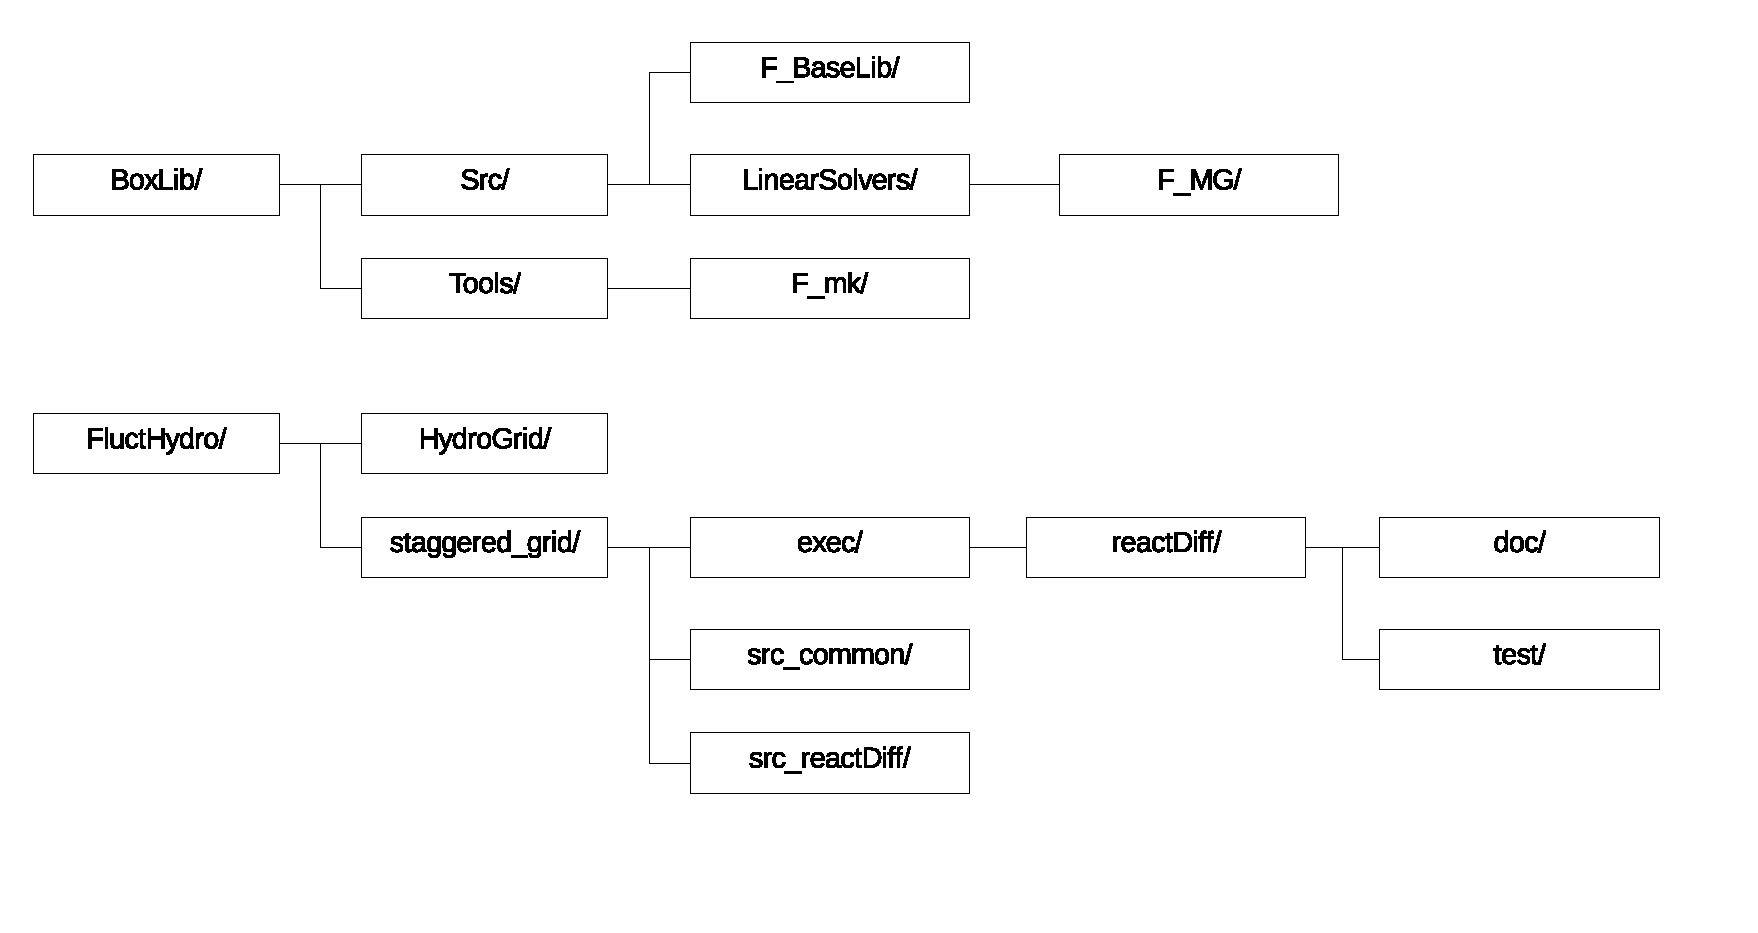
\includegraphics[width=6in]{./directory}
\caption{\label{fig:directory}Directory structure.}
\end{figure}
%%%%%%%%%%%%%%%%%%%%%%%%%%%%%%%%%%%%%
\begin{itemize}

\item {\tt BoxLib/}

\begin{itemize}

\item {\tt Src/}

\begin{itemize}

\item {\tt F\_BaseLib/}

Core libraries for parallelization of structured grid data.

\item {\tt LinearSolvers/F\_MG/}

Core libraries for linear solvers (for implicit diffusion) and diffusion stencils.

\end{itemize}
\end{itemize}

\begin{itemize}

\item {\tt Tools/F\_mk/}

Make system variables and flags.

\end{itemize}
\end{itemize}

\begin{itemize}

\item {\tt FluctHydro/}

\begin{itemize}

\item {\tt HydroGrid/}

\item {\tt staggered\_grid/}

\begin{itemize}

\item {\tt exec/reactDiff/doc/}

Contains the document you are reading right now!

\item {\tt exec/reactDiff/test/}

This is the compilation directory.  Contains a GNUmakefile and inputs files.

\item {\tt src\_common/}

Source code shared by all our staggered grid codes.  Contains generic namelist parameters
and routines for boundary conditions, divergence, etc.

\item {\tt src\_reactDiff/}

Source code specific to this reaction/diffusion problem.

\end{itemize}
\end{itemize}
\end{itemize}

\subsection{Compiling and Running}
Go to {\tt FluctHydro/staggered\_grid/exec/reactDiff/test/} and edit the 
{\tt GNUmakefile} settings to your liking (below) and simply type {\tt `make'}.\\
\begin{verbatim}
NDEBUG    :=           # 'not debug'.  use 't' for an optimized build
MPI       := t         # use 't' to build an mpi executable
OMP       :=           # use 't' to build an OpenMP threadded executable
PROF      :=           # use 't' to turn on code profiling
COMP      := gfortran  # fortran compiler
CCOMP     := gcc       # c compiler
MKVERBOSE := t         # make verbosity

\end{verbatim}
This will generate an executable whose name provides information about the build settings,
i.e., what compiler was used, whether MPI and/or OpenMP were enabled, etc.
To run the code, simply type the executable name, followed by an inputs file.

\subsection{Input Parameters}
Refer to {\tt src\_common/probin\_common.f90} and 
{\tt src\_reactDiff/probin\_reactDiff.f90} for namelist parameters used in the
simulation and an explanation of what the parameters do.  Note that only a subset
of the parameters in {\tt probin\_common.f90} are used in this code.

\section{Algorithms}
\subsection{Spatial Discretization}
We use a finite volume framework on a regular Cartesian mesh with grid spacing $\Delta x$.
The number densities are assumed to be the average over the cell.
We assume the Fickean diffusion coefficients, $D_k$ are constant, but these can be generalized
in future releases to be function of space, time, and/or composition.

The deterministic diffusion terms are spatially discretized using the standard 5-point (in 2D) or
7-point (in 3D) variable-coefficient Laplacian, e.g.,
\begin{eqnarray}
\nabla\cdot D\nabla n &\rightarrow& \frac{1}{\Delta x}\left[D_{i+\half,j}\left(\frac{n_{i+1,j}-n_{i,j}}{\Delta x}\right) - D_{i-\half,j}\left(\frac{n_{i,j}-n_{i-1,j}}{\Delta x}\right)\right] \nonumber\\
&& + \frac{1}{\Delta x}\left[D_{i,j+\half}\left(\frac{n_{i,j+1}-n_{i,j}}{\Delta x}\right) - D_{i,j-\half}\left(\frac{n_{i,j}-n_{i,j-1}}{\Delta x}\right)\right]. \nonumber\\
\end{eqnarray}
The stochastic diffusion terms use the standard divergence,
\begin{eqnarray}
\nabla\cdot\sqrt{2Dn}\mZb &\rightarrow&\left[\frac{\sqrt{2D_{i+\half,j}n_{i+\half,j}}\mathcal{Z}_{i+\half,j} - \sqrt{2D_{i-\half,j}n_{i-\half,j}}\mathcal{Z}_{i-\half,j}}{\Delta x}\right]\nonumber\\
&&+ \left[\frac{\sqrt{2D_{i,j+\half}n_{i,j+\half}}\mathcal{Z}_{i,j+\half} - \sqrt{2D_{i,j-\half}n_{i,j-\half}}\mathcal{Z}_{i,j-\half}}{\Delta x}\right]
\end{eqnarray}
To obtain diffusion coefficients or number densities on faces, there are several options for averaging the neighboring cell-averaged data to faces.  These include a variety of arithmetic, geometric, and harmonic stencils with options for preventing negative number densities using smoothing functions.  See the subroutine {\tt average\_values} in {\tt average\_to\_faces.f90} for current implementation.

\subsection{Boundary Conditions}
The code supports periodic, solid wall ($\partial n_k/\partial t = g_k$), and reservoir 
($n_k = f_k$) boundary conditions using standard first-order stenciles at the boundary.

\subsection{Temporal Discretization}
Consider PDEs describing
diffusion and reactions in isolation:
\begin{equation}
\frac{\partial n_k}{\partial t} = \nabla\cdot\left(D_k\nabla n_k + \sqrt{\frac{2D_kn_k}{A}}\mZb\right),\label{eq:Diffusion}
\end{equation}
\begin{equation}
\frac{\partial n_k}{\partial t} = \mRb(\nb).\label{eq:Reactions}
\end{equation}
The code supports three temporal splitting schemes:\\

{\bf First-Order Temporal Splitting:}
(($\Delta t R$)($\Delta t D$))
\begin{enumerate}
\item Advance $\nb^n \rightarrow \nb^{(1)}$ by discretizing 
diffusion (\ref{eq:Diffusion}) over $\Delta t$.
\item Advance $\nb^{(1)} \rightarrow \nb^{n+1}$ by discretizing 
reactions (\ref{eq:Reactions}) over $\Delta t$.
\end{enumerate}

{\bf Second-Order Strang Splitting, Option 1:}
(($\frac{\Delta t}{2}R$)($\Delta t D$)($\frac{\Delta t}{2}R$))
\begin{enumerate}
\item Advance $\nb^n \rightarrow \nb^{(1)}$ by discretizing 
reactions (\ref{eq:Reactions}) over $\Delta t/2$.
\item Advance $\nb^{(1)} \rightarrow \nb^{(2)}$ by discretizing 
diffusion (\ref{eq:Diffusion}) over $\Delta t$.
\item Advance $\nb^{(2)} \rightarrow \nb^{n+1}$ by discretizing 
reactions (\ref{eq:Reactions}) over $\Delta t/2$.
\end{enumerate}

{\bf Second-Order Strang Splitting, Option 2:}
(($\frac{\Delta t}{2}D$)($\Delta t R$)($\frac{\Delta t}{2}D$))
\begin{enumerate}
\item Advance $\nb^n \rightarrow \nb^{(1)}$ by discretizing 
diffusion (\ref{eq:Diffusion}) over $\Delta t/2$.
\item Advance $\nb^{(1)} \rightarrow \nb^{(2)}$ by discretizing 
reactions (\ref{eq:Reactions}) over $\Delta t$.
\item Advance $\nb^{(2)} \rightarrow \nb^{n+1}$ by discretizing 
diffusion (\ref{eq:Diffusion}) over $\Delta t/2$.
\end{enumerate}

\subsection{Diffusion}
The Fickean diffusion term is discretized using standard finite volume
Laplacian-like stencils:
\begin{equation}
\nabla\cdot D\nabla n \rightarrow \sum_d \frac{1}{\Delta x}\left[D_{\ib+\half\eb_d}\left(\frac{n_{\ib + \eb_d}-n_{\ib}}{\Delta x}\right) - D_{\ib-\half\eb_d}\left(\frac{n_{\ib}-n_{\ib-\eb_d}}{\Delta x}\right)\right],\label{eq:diffusion_stencil}
\end{equation}
For the stochastic fluxes,
we generate random $\mZb$ on faces directory, compute $n$ on faces
using either arithmetic, geometric, or harmonic averaging from the 
neighboring cell centers, and use the same stencil 
in (\ref{eq:diffusion_stencil}).
When a cell has a negative density, stochastic fluxes through the faces of the cell are zeroed in all three average types.
For the arithmetic-mean average type, a smoothed Heaviside function is employed so that the flux can be continuous as a function of the number densities of two contiguous cells. 
\\

In order to discretize the diffusion equation (\ref{eq:Diffusion}) over a time 
increment $\delta t$, we have three options.  We use the superscripts $n$
and $n+1$ to denote the state at $t^n$ and $t^{n+1}=t^n+\delta t$, noting
that $\delta t$ can be a fraction of the time step $\Delta t$.\\

{\bf Explicit Predictor-Corrector}
We use a single set of random numbers, and keep the noise amplitude
fixed (Ito interpretation):
\begin{equation}
n_k^{n+1,*} = n_k^n + \delta t \nabla\cdot\left(D_k \nabla n_k^n
+ \sqrt{\frac{2 D_k n_k^n}{\delta t\Delta V}}\mZb^{(1)}\right),
\end{equation}
\begin{equation}
n_k^{n+1} = n_k^n + \delta t\nabla\cdot\left(
\half D_k\nabla n_k^n + \half D_k\nabla n_k^{n+1,*}
+ \sqrt{\frac{2 D_k n_k^n}{\delta t\Delta V}}\mZb^{(1)}
\right).
\end{equation}

{\bf Crank-Nicolson}
We update the number densities using a single semi-implicit solve:
\begin{equation}
n_k^{n+1} = n_k^n + \delta t\nabla\cdot\left(
\half D_k\nabla n_k^n + \half D_k\nabla n_k^{n+1}
+ \sqrt{\frac{2 D_k n_k^n}{\delta t\Delta V}}\mZb^{(1)}
\right),
\end{equation}
i.e.,
\begin{equation}
\left(\mathcal{I} - \nabla\cdot\frac{\delta t}{2}D_k\nabla\right)n_k^{n+1} = 
n_k^n + \delta t\nabla\cdot\left(\half D_k\nabla n_k^n
+ \sqrt{\frac{2 D_k n_k^n}{\delta t\Delta V}}\mZb^{(1)}\right).
\end{equation}
In practice, we define $n_k^{n+1} = n_k^n + \delta n_k$ and rewrite the implicit
system in ``delta'' form,
\begin{equation}
\left(\mathcal{I} - \nabla\cdot\frac{\delta t}{2}D_k\nabla\right)\delta n_k = 
\delta t\nabla\cdot\left(D_k\nabla n_k^n + \sqrt{\frac{2 D_k n_k^n}{\delta t\Delta V}}\mZb^{(1)}\right),
\end{equation}
and then set $n_k^{n+1} = n_k^n + \delta n_k$.\\

{\bf Explicit Midpoint}
We use two sets of random numbers, but use the same noise amplitude for both:
\begin{equation}
n_k^{n+\myhalf} = n_k^n + \frac{\delta t}{2} \nabla\cdot\left(D_k\nabla n_k^n
+ \sqrt{\frac{2 D_k n_k^n}{(\delta t/2)\Delta V}}\mZb^{(1)}\right),
\end{equation}
\begin{equation}
n_k^{n+1} = n_k^n + \delta t\nabla\cdot\left(
D_k\nabla n_k^{n+\myhalf}
+ \sqrt{\frac{2 D_k n_k^n}{\delta t\Delta V}}\left(\frac{\mZb^{(1)}+\mZb^{(2)}}{\sqrt{2}}\right)
\right).
\end{equation}
Note that there are other options which should be considered as well. One of them is to generate separate
stochastic mass fluxes for the two halves of the time step:
\begin{equation}
n_k^{n+1} = n_k^n + \delta t\nabla\cdot\left(
D_k\nabla n_k^{n+\myhalf}
+ \sqrt{\frac{2 D_k n_k^n}{\delta t\Delta V}} \frac{\mZb^{(1)}}{\sqrt{2}}
+ \sqrt{\frac{2 D_k n_k^{n+\myhalf}}{\delta t\Delta V}} \frac{\mZb^{(2)}}{\sqrt{2}}\right).
\end{equation}
Another alternative that fits well in the predictor-corrector algorithm proposed in \cite{AndersonMattingly2011}
is
\begin{equation}
n_k^{n+1} = n_k^n + \delta t\nabla\cdot\left(
D_k\nabla n_k^{n+\myhalf}
+ \sqrt{\frac{2 D_k n_k^n}{\delta t\Delta V}} \frac{\mZb^{(1)}}{\sqrt{2}}
+ \sqrt{\frac{2 D_k \left( 2 n_k^{n+\myhalf} - n_k^n \right)^+ }{\delta t\Delta V}} \frac{\mZb^{(2)}}{\sqrt{2}}\right).
\end{equation}

\subsection{Reactions}
In order to discretize the reaction equation (\ref{eq:Reactions}) over a time
increment $\delta t$, we have three options: stochastic
simulation algorithm (SSA), tau-leaping, and chemical Langevin equation (CLE).
See \cite{Gillespie2007} for an overview of these methods.  We have options
for second-order tau-leaping and CLE using the predictor-corrector
method in \cite{AndersonMattingly2011}.\\

Our stochastic reactions require deterministic reaction rates, which we obtain
using the law of mass action.  Define $a_i(\nb)$ as the deterministic reaction
rate in units of (?) for reaction $i$, and $a_0(\nb) = \sum a_i(\nb)$.\\

{\bf SSA}.  To summarize, if we assume each reaction is a Poisson process, we
can generate the time that the next reaction will occur using a uniform random
variable, and then determine which reaction occurred using a separate 
uniform random variable.  Then, update the state and repeat.\\

{\bf Tau Leaping}\\

{\bf CLE}

\section{Unsplitting Schemes}

%%%%%%%%%%%%%%%%%%%%%%%%%%%%%%%%%%%%%%%%%%%%%%%%%%%%%%%%%%%%%%%%%%%%%%%%%%%%%%%%

\newcommand{\Pc}{\mathcal{P}}           % mathcal P
\newcommand{\Nc}{\mathcal{N}}           % mathcal N 
\newcommand{\Rfrak}{\mathfrak{R}}       % fraktur R
\newcommand{\nablab}{\bm{\nabla}}       % nabla in boldface

\newcommand{\dt}{{\Delta t}}            % Delta t 
\newcommand{\dthalf}{{\frac{\dt}{2}}}   % dt/2 (frac)
\newcommand{\dV}{{\Delta V}}            % Delta V 

\newcommand{\Ns}{{N_\mathrm{s}}}        % number of species
\newcommand{\Nr}{{N_\mathrm{r}}}        % number of reactions
\newcommand{\Ds}{{D_s}}                 % diffusion coefficient of species s
\newcommand{\ns}{n_s}                   % number density of species s
\newcommand{\ar}{a_r}                   % reaction rate of reaction r
\newcommand{\tar}{{\ta_r}}              % LMA-corrected reaction rate of r
\newcommand{\nusr}{{\nu_{s r}}}         % stoichiometric factor of s in r
\newcommand{\tn}{\tilde{n}}             % tilde n (for avg_type)
\newcommand{\ta}{\tilde{a}}             % tilde a (for LMA correction)
\newcommand{\pone}{{(1)}}               % 1 in parentheses
\newcommand{\ptwo}{{(2)}}               % 2 in parentheses

%%%%%%%%%%%%%%%%%%%%%%%%%%%%%%%%%%%%%%%%%%%%%%%%%%%%%%%%%%%%%%%%%%%%%%%%%%%%%%%%

\subsection{Reaction}

Depending on the value of \texttt{use\_Poisson\_rng}, one of the following four methods is employed to sample the reaction:

\begin{center}
\begin{tabular}{|c|c|}
\hline 
\texttt{use\_Poisson\_rng} & sampling method \\
\hline
2 & SSA \\
1 & tau-leaping (Poissonian increment) \\
0 & CLE (Gaussian increment) \\
-1 & deterministic \\
\hline
\end{tabular}
\end{center}
For the SSA, the change in $\ns$ after time $\tau$ for initial state $\nb$ is denoted by $\Rfrak_s(\nb,\tau)$.
For the other methods, the number of occurrences of reaction $r$ per volume during time interval $\tau$ is denoted by $R_r(a_r,\tau)$.
This is sampled as follows:
\begin{equation}
R_r(\ar,\tau)=\begin{cases}
\frac{1}{\dV}\Pc(\ar\dV\tau)  & \mbox{for tau-leaping}, \\
\ar\tau+\sqrt{\frac{\ar\tau}{\dV}}\Nc(0,1) & \mbox{for CLE}, \\
\ar\tau & \mbox{for deterministic},
\end{cases}
\end{equation}
and the change in $\ns$ is obtained from $\sum_{r=1}^\Nr \nusr R_r (\ar,\tau)$.
Here, $\ar=\ar(\nb)$ is the deterministic reaction rate of reaction $r$ and $\nusr$ is the stoichiometric factor of species $s$ in reaction $r$;
$\Pc(\lambda)$ and $\Nc(0,1)$ are the Poisson distribution with mean $\lambda$ and the standard normal distribution, respectively.
Note that the integer-based LMA, $\tar$, can be used by setting \texttt{include\_discrete\_LMA\_correction = T}.

In the subsequent subsections, we present the unsplitting schemes implemented in the codes.
Note that the CLE or deterministic case has the same temporal integrator form as the tau-leaping case.
In addition, as in the previous section, all midpoint schemes have three possibilities for the calculation of the stochastic diffusive flux for the second-half step.
That is, $\tn_s^\bullet$ can be $\ns^k$, $\ns^\star$, or $(2\ns^\star-\ns^k)^+$.

\subsection{Forward Euler Scheme}

For the tau-leaping reaction, the scheme is written as
\begin{equation}
\ns^{k+1} = \ns^k + \dt\Ds\nablab^2\ns^k
+\sqrt{\frac{2\Ds\tn_s^k}{\dV}\dt} \nablab\cdot Z_s^\pone
+\sum_{r=1}^\Nr \nusr R_r^\pone\left(\ar^k,\dt\right).
\end{equation}
For the SSA case, the reaction part is simply replaced by $\Rfrak_s^\pone\left(\nb^k,\dt\right)$.

\subsection{Multinomial diffusion}

Similar to the forward Euler scheme except that the change due to diffusion is calculated from the multinomial diffusion.  

\subsection{Explicit Midpoint + Tau-Leaping Scheme}

By combining the explicit midpoint scheme for diffusion given in the previous section
with the $\theta$-trapezoidal $\tau$-leaping scheme proposed in Ref.~\cite{HuLiMin2011} with $\theta=\frac{1}{2}$,
we obtain the following scheme:
\begin{subequations}
\begin{align}
&\ns^\star = \ns^k + \dthalf\Ds\nablab^2\ns^k 
+\sqrt{\frac{2\Ds\tn_s^k}{\dV}\dthalf} \nablab\cdot Z_s^\pone
+\sum_{r=1}^\Nr \nusr R_r^\pone\left(\ar^k,\dthalf\right),\\
&\ns^{k+1} = \ns^k + \dt\Ds\nablab^2\ns^\star
+\sqrt{\frac{2\Ds\tn_s^k}{\dV}\dthalf} \nablab\cdot Z_s^\pone
+\sqrt{\frac{2\Ds\tn_s^\bullet}{\dV}\dthalf} \nablab\cdot Z_s^\ptwo\\
&\quad+\sum_{r=1}^\Nr \nusr R_r^\pone\left(\ar^k,\dthalf\right)
+\sum_{r=1}^\Nr \nusr R_r^\ptwo\left((2\ar^\star-\ar^k)^+,\dthalf\right)\notag
\end{align}
\end{subequations}

\subsection{Explicit Midpoint + SSA Scheme}

\begin{subequations}
\begin{align}
&\ns^{\star\star} = \ns^k + \dthalf\Ds\nablab^2\ns^k 
+\sqrt{\frac{2\Ds\tn_s^k}{\dV}\dthalf} \nablab\cdot Z_s^\pone,\\
&\ns^\star = \ns^{\star\star} + \Rfrak_s^\pone\left(\nb^{\star\star},\dthalf\right),\\
&\ns^{k+1} = n_s^k + \dt\Ds\nablab^2 n_s^\star
+\sqrt{\frac{2\Ds\tn_s^k}{\dV}\dthalf} \nablab\cdot Z_s^\pone
+\sqrt{\frac{2\Ds\tn_s^\bullet}{\dV}\dthalf} \nablab\cdot Z_s^\ptwo\\
&\quad+\Rfrak_s^\pone\left(\nb^{\star\star},\dthalf\right)
+\Rfrak_s^\ptwo\left(\nb^\star,\dthalf\right)\notag
\end{align}
\end{subequations}

\subsection{Implicit Midpoint + Tau-Leaping Scheme}

While we use a backward-Euler-type stepping for the predictor stage $\nb^\star$, we use a Crank--Nicolson-type stepping for the corrector stage $\nb^{k+1}$.
\begin{subequations}
\begin{align}
&\ns^\star = \ns^k + \dthalf\Ds\nablab^2\ns^\star
+\sqrt{\frac{2\Ds\tilde{n}_s^k}{\dV}\dthalf}\nablab\cdot Z_s^\pone
+\sum_{r=1}^\Nr \nusr R_r^\pone\left(\ar^k,\dthalf\right),\\
&\ns^{k+1} = \ns^k + \dt\Ds\nablab^2 \left[\frac{n_s^k+n_s^{k+1}}{2}\right]
+\sqrt{\frac{2\Ds\tn_s^k}{\dV}\dthalf} \nablab\cdot Z_s^\pone
+\sqrt{\frac{2\Ds\tn_s^\bullet}{\dV}\dthalf} \nablab\cdot Z_s^\ptwo\\
&\quad+\sum_{r=1}^\Nr \nusr R_r^\pone\left(\ar^k,\dthalf\right)
+\sum_{r=1}^\Nr \nusr R_r^\ptwo\left((2\ar^\star-\ar^k)^+,\dthalf\right)\notag
\end{align}
\end{subequations}

\subsection{Implicit Midpoint + SSA Scheme}

\begin{subequations}
\begin{align}
&\ns^\star = \ns^k + \dthalf\Ds\nablab^2\ns^\star
+\sqrt{\frac{2\Ds\tn_s^k}{\dV}\dthalf} \nablab\cdot Z_s^\pone,\\
&\ns^{k+1} = \ns^k + \dt\Ds\nablab^2 \left[\frac{n_s^k+n_s^{k+1}}{2}\right]
+\sqrt{\frac{2\Ds\tn_s^k}{\dV}\dthalf} \nablab\cdot Z_s^\pone
+\sqrt{\frac{2\Ds\tn_s^\bullet}{\dV}\dthalf} \nablab\cdot Z_s^\ptwo
+\Rfrak_s^\pone\left(\nb^\star,\dt\right)
\end{align}
\end{subequations}

\section{Inhomogeneous Boundary Conditions}
In order to handle inhomogeneous boundary conditions correctly within a second-order
splitting scheme, we use \cite{Einkemmer:2014}.  We first consider second-order
Strang Splitting, Option 2 (($\frac{\Delta t}{2}D$)($\Delta t R$)($\frac{\Delta t}{2}D$)).
The diffusion and reaction solvers need to be modified to include an external, 
constant-in-time forcing terms, $F_d$ and $F_r$.

This algorithm assumes the boundary conditions are independent of time.  This
assumption can be changed later.  The stochastic reactions and diffusive fluxes
probably aren't treated right in this description yet.

\begin{itemize}
\item Compute $\nabla\cdot D_k\nabla n_k^{\rm steady} = 0$ with inhomogeneous number density boundary
conditions.

\item Compute deterministic reaction rates, $\Rb(\nb^{\rm steady})$.
\end{itemize}

Then use any of the splitting schemes above, but with an additional piecewise-constant
source term:
\begin{equation}
\frac{\partial n_k}{\partial t} = \nabla\cdot\left(D_k\nabla n_k + \sqrt{\frac{2D_kn_k}{A}}\mZb\right) + \Rb(\nb^{\rm steady}),\label{eq:Diffusion_bc}
\end{equation}
\begin{equation}
\frac{\partial n_k}{\partial t} = \mRb(\nb) - \Rb(\nb^{\rm steady}).\label{eq:Reactions_bc}
\end{equation}
For stochastic reactions with multiple stages, we may want to include the source 
term contribution at intermediate stages.

\bibliographystyle{plain}
\bibliography{DesignDocument}

\end{document}
